\section{Application aux données réelles : aiguillage}
L'analyse porte sur quatre classes. Les transitions de la colonne 553 donnent
les coupures Python $[35,75,120]$ ; en numérotation à partir de 1, les débuts
des nouveaux segments sont $[36,76,121]$. Fisher retrouve exactement ces limites
et les effectifs $[35,40,45,20]$.

\begin{figure}[H]
\centering
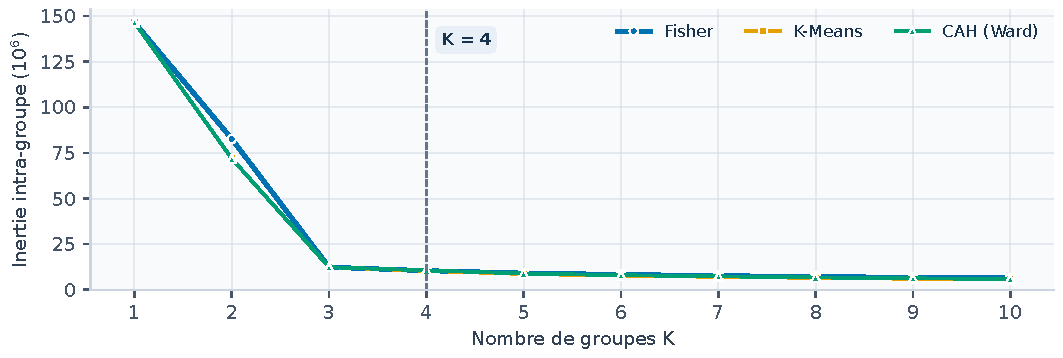
\includegraphics[width=0.94\linewidth,height=4.5cm,keepaspectratio]{aiguillage_coude.pdf}
\caption[Aiguillage : inerties selon le nombre de classes]{Inerties sur \file{aiguillage}. Le trait vertical indique $K=4$,
fixé pour la comparaison avec les quatre classes de référence.}
\label{fig:reelcourbes}
\end{figure}
La décroissance ralentit nettement après $K=3$
(figure~\ref{fig:reelcourbes}). Les quatre classes sont ici connues :
$K=4$ sert à évaluer leur reconstitution, indépendamment de ce coude.

\begin{table}[H]
\centering\small
\begin{tabular}{lrrrr}
\toprule
Méthode & ARI & Corrects & TBC & Changements \\
\midrule
Fisher & 1{,}000 & 140/140 & 100{,}00\,\% & 3 \\
K-Means & 0{,}943 & 137/140 & 97{,}86\,\% & 9 \\
CAH (Ward) & 0{,}859 & 132/140 & 94{,}29\,\% & 7 \\
\bottomrule
\end{tabular}

\caption[Aiguillage : ARI, TBC et changements de label]{Résultats sur les 140 observations, dans l'espace brut à 552 variables.
Le TBC suit l'alignement optimal ; K-means utilise 20 départs, graine 42.}
\label{tab:reel}
\end{table}

\begin{figure}[H]
\centering
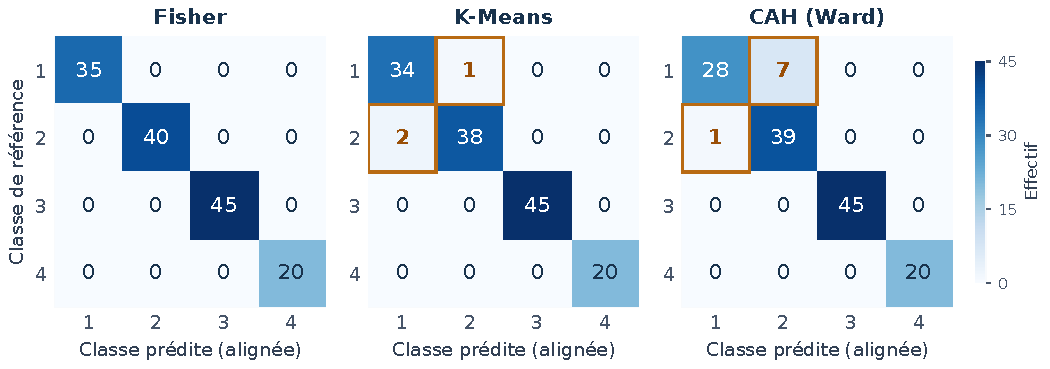
\includegraphics[width=0.98\linewidth,height=5.5cm,keepaspectratio]{aiguillage_confusion.pdf}
\caption[Aiguillage : matrices de confusion]{Matrices de confusion après permutation optimale des labels.
Les lignes sont les classes de référence ; les colonnes, les classes prédites.
L'échelle de couleur est commune ; les cellules encadrées signalent les erreurs.}
\label{fig:confusion}
\end{figure}

Les erreurs se lisent directement dans la figure~\ref{fig:confusion}.
Fisher classe les 140 observations conformément à la référence.
Les K-means affectent une observation de la classe 1 à la classe 2 et deux
dans le sens inverse : 137 observations sont correctement affectées.
Ward confond sept observations de la classe 1 avec la classe 2 et une dans
le sens inverse, soit 132 bonnes affectations. Les classes 3 et 4 sont
intégralement retrouvées par les trois méthodes.

\begin{figure}[H]
\centering
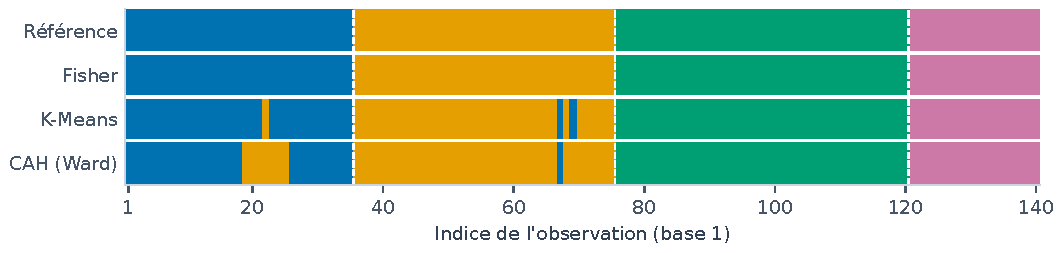
\includegraphics[width=0.98\linewidth,height=3.2cm,keepaspectratio]{aiguillage_ordre.pdf}
\caption[Aiguillage : labels selon l'ordre d'acquisition]{Labels selon l'ordre d'acquisition. Une même couleur représente la
même classe alignée dans les quatre lignes ; les pointillés séparent les
segments retrouvés par Fisher.}
\label{fig:ordre}
\end{figure}

La figure~\ref{fig:ordre} montre que les erreurs des comparateurs introduisent
des allers-retours entre les deux premiers régimes. Les K-means ont un meilleur
TBC que Ward, mais davantage de changements de label (9 contre 7) : l'accord
à la référence et la continuité temporelle ne sont donc pas équivalents.

\begin{figure}[H]
\centering
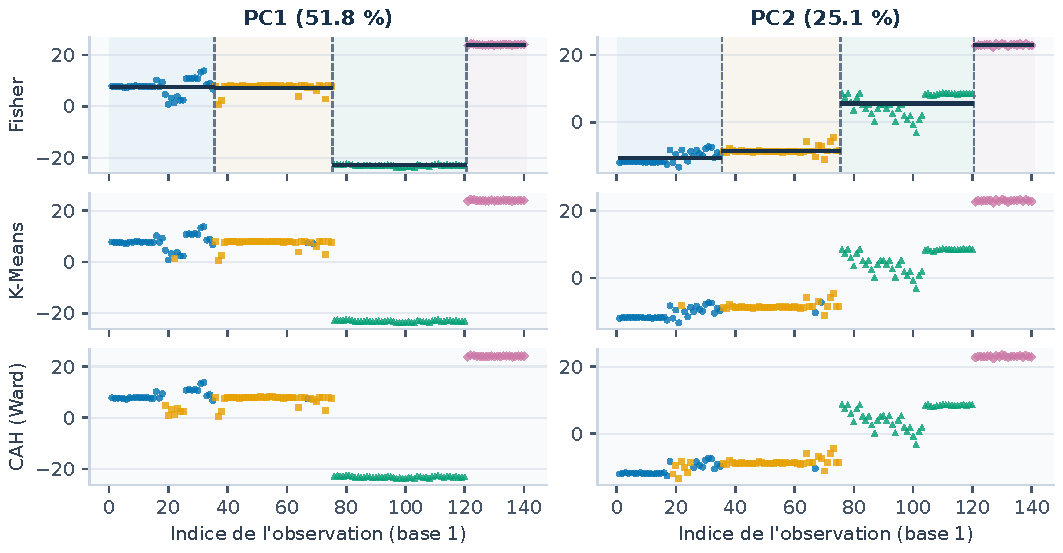
\includegraphics[width=0.98\linewidth,height=7.4cm,keepaspectratio]{aiguillage_temps.pdf}
\caption[Aiguillage : composantes principales selon l'ordre]{PC1 et PC2 selon l'indice d'observation. Les pointillés délimitent les
segments Fisher ; les traits horizontaux indiquent leurs moyennes projetées.
Les couleurs sont alignées sur la référence. L'ACP centrée-réduite sert à
l'affichage ; les partitions sont ajustées sur les 552 variables brutes.}
\label{fig:reeltemps}
\end{figure}
Les moyennes par segment dans la figure~\ref{fig:reeltemps} rendent visibles
les régimes successifs dans cette projection.

La décomposition de Huygens $I=I_W+I_B$ \cite{same} est vérifiée
numériquement. L'inertie et l'accord à la référence restent deux critères distincts :
les K-means ont une inertie de $10{,}346\times10^6$, contre
$10{,}458\times10^6$ pour Fisher et $10{,}599\times10^6$ pour Ward,
sans retrouver tous les labels.
Les K-means peuvent réduire la dispersion en regroupant des observations non
contiguës ; l'inertie seule ne mesure donc pas l'accord à la référence.
